Проведём два вектора $\vc{r}_A, \vc{r}_O$:
\begin{equation*}
    \vc{r}_A = \vc{r}_O + \vc{r} = \vc{r}_O + R(t) \vc{\rho}
    \hspace{0.5cm} \overset{d / dt}{\Rightarrow} \hspace{0.5cm} 
    \vc{v}_A = \vc{v}_O + \dot{R} \rho = \vc{v}_O + \dot{R} R^{-1}\vc{r}
\end{equation*}
но,
\begin{equation*}
    RR\T = E, \dot{R} R\T + R \dot{R}\T = 0, \dot{R} R\T = - R \dot{R}\T,
    (\dot{R} R^{-1})\T = - \dot{R} R^{-1}.
\end{equation*}

То есть $\dot{R} R^{-1}$ кососимметрична. Тогда пусть
\begin{equation*}
    \dot{R} R^{-1} = \Omega = \begin{pmatrix}
        0 & -\omega_z & w_y \\
        w_z & 0 & -\omega_x \\
        -\omega_y & \omega_x & 0\\
    \end{pmatrix}
\end{equation*}
Таким образом мы доказали следующую теорему.

\begin{to_thr}[формула Эйлера]
\label{eq_euler}
    Существует единственный вектор\footnote{
        Псевдоветор же, нет?
    } $\vc{\omega}$, называемый \textbf{угловой скоростью тела}, с помощью которого скорость $\vc{v}$ точки тела может быть представлена в виде
    \begin{equation*}
        \vc{v}_A = \vc{v}_O + \vc{\omega} \times \vc{r}
        \hspace{0.5cm} \text{--} \hspace{0.5cm} \text{\textbf{формула Эйлера}.}
    \end{equation*}
\end{to_thr}

Тогда, например, при постоянном радиус векторе верно, что
\begin{equation*}
    \vc{v}_A = \frac{d \vc{a}}{dt} = \vc{\omega} \times \vc{a},
    \hspace{0.5cm} \text{при условии $a = \const$}.
\end{equation*}

Можно вывести ускорение точки твёрдого тела
\begin{align*}
    \vc{\mathrm{w}}_A &= \vc{\mathrm{w}}_O + \frac{d \vc{\omega}}{dt} \times \vc{r} + \vc{\omega} \times \frac{d \vc{r}}{dt}, \\
    \vc{\mathrm{w}}_A &= \vc{\mathrm{w}}_O + \vc{\varepsilon} \times \vc{r} + \vc{\omega} \times \left(\vc{\omega} \times \vc{r} \right)
    \hspace{0.5cm} \text{--} \hspace{0.5cm} \text{\textbf{формула Ривальса},}
\end{align*}
где $\vc{\varepsilon} = d \vc{\omega} / d t$ -- \textit{угловое ускорение}.

\subsubsection*{Вращение вокруг неподвижной оси}
\begin{wrapfigure}{r}{0.25\textwidth}
  \begin{center}
        \vspace{-10 mm}
        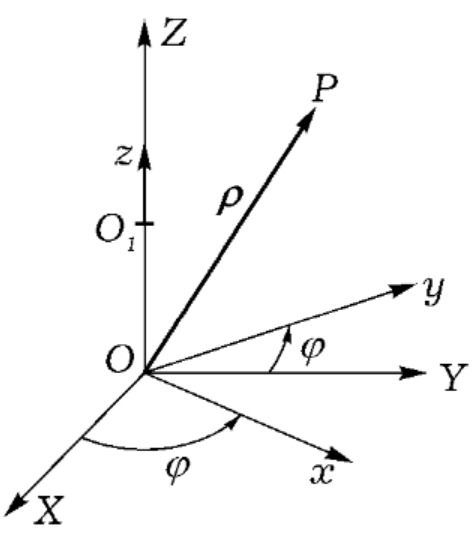
\includegraphics[width=0.9\linewidth]{img/stable_axis.png}
  \end{center}
    \caption{Ориентация тела относительно неподвижной системы координат}
\end{wrapfigure}
Пусть точка $P$ задана в связанной системе координат радиус-вектором $\rho$:
\begin{equation*}
    \vc{r} = A \vc{\rho},
    \hspace*{0.5 cm}
    A = \begin{pmatrix}
            \cos \varphi & - \sin \varphi & 0 \\
            \sin \varphi & \cos \varphi & 0 \\
            0 & 0 & 1
        \end{pmatrix}.
\end{equation*}
После прямых вычислений получаем, что
\begin{equation*}
    \dot{A} A^{-1} = 
    \begin{pmatrix}
        0 & - \dot{\varphi} & 0 \\
        \dot{\varphi} & 0 & 0 \\
        0 & 0 & 0    
    \end{pmatrix},
    \hspace*{1 cm}
    \dot{\omega} = \begin{pmatrix}
        0 \\ 0 \\ \dot{\varphi}
    \end{pmatrix},
    \hspace*{1 cm}
    \vc{\varepsilon} = \begin{pmatrix}
        0 \\ 0 \\ \ddot{\varphi}    
    \end{pmatrix}.
\end{equation*}
Таким образом получили, что угловая скорость $\vc{\omega}$ направлена по оси вращения по правилу буравчика. Угловое ускорение $\vc{\varepsilon}$ коллинеарно $\vc{\omega}$.

Для вычисления $w_P$ примем $O$ за полюс. Тогда $v_O= 0$, что значит $\vc{v} = \vc{\omega} \times \vc{r}$ -- вектор скорости перпендикулярен оси вращения. И из формулы Ривальса:
\begin{equation*}
    w = \underbrace{\vc{\varepsilon} \times \vc{r}}_{w_\text{вр}} + \underbrace{\vc{\omega} \times \vc{v}}_{w_\text{ос}},
    \hspace*{1 cm}
\end{equation*}
где \textit{вращательное} ускорение $w_\text{вр} = \ddot{|\varphi}| d$, а \textit{осестремительное} $w_\text{ос} = \omega^{2}d$, а $d$ --- радиус окружности, по которой движется $P$.

\subsubsection*{Движение вокруг неподвижной точки}
Точка $O$ --- неподвижна, тогда $v_0 = 0, \ w_0 = 0 $ и формулы, полученные в разделе выше одни и те же. Однако стоит ввести пару определений:
\begin{to_def}
    \textit{Мгновенная ось вращения} --- ось на которой в данный момент времени лежит $\vc{\omega}$, которая в свою очередь --- \textit{мгновенная угловая скорость}. 
\end{to_def}
\begin{to_def}
    При своём движении мгновенная ось вращения описывает в теле коническую поверхность --- \textit{подвижный аксоид}, а в абсолютном пространстве --- \textit{неподвижный аксоид}.
    При движении тела подвижный аксоид катится по неподвижному без скольжения.
\end{to_def}

Годограф $\vc{\omega}$ лежит на неподвижном аксоиде. 
Так как $\vc{\varepsilon} = \vc{\dot{\omega}}$, то $\vc{\varepsilon}$ направлено по касательной к годографу и вовсе не обязательно по мгновенной оси вращения. 
Если $\vc{\omega} = \omega \vc{e}$, для единичного $\vc{e}$, то $\vc{\varepsilon} = \dot{\omega} \vc{e} +\omega \vc{\dot{e}}$.
Если мгновенная ось вращается вокруг $O$ с $\vc{\Omega}$, то $\omega \vc{\dot{e}} = \vc{\Omega} \times \vc{\omega}$.

Вновь воспользовавшись формулой Ривальса вычислим осетремительное ускорение, для $Q$ --- точке на мгновенной оси вращения:
\begin{equation*}
    w_\text{ос} = \vc{\omega}\times (\vc{\omega} \times \vc{r}) = \omega^2 \vc{e} \times (\vc{e} \times \vc{r}) = \omega^2[\vc{e} (\vc{e} \cdot \vc{r}) - \vc{r}] = \omega^2 (\overrightarrow{O Q} - \vc{r}) = \omega^2 \vc{l}.
\end{equation*}
Таким образом получили, что $w_\text{ос}$ совпадает при вращении, как если бы ось было неподвижной.

\subsubsection*{Плоское движение}
\begin{to_def}
    \textit{Плоское движение} --- движение тела, при котором все его точки перемещаются в плоскостях параллельных некоторой неподвижной плоскости.
\end{to_def}

Плоская фигура вынужденно двигаясь в своей плоскости имеет три степени свободы: $(x,y,\varphi)$. Скорости и ускорения всё так же ищутся по общем формулам, но в данном случае полезно рассмотреть несколько теорем:
\begin{to_thr}
    При плоском движении фигуры во мгновение $t$, если движение не поступательно, то $\exists ! C$-точка, такая что $v_C =0$, а остальные точки тела движутся как при вращении вокруг $C$.
\end{to_thr}
\begin{to_def}
    Такая точка $C$ --- называется \textit{мгновенным центром скоростей}.
\end{to_def}

\begin{to_thr}
    Для движения плоской фигуры в своей плоскости. Если в момент $t$ $\dot{\varphi} \neq 0 || \ddot{\varphi} \neq 0$, то в $t$ $\exists ! Q$-точка фигуры, такая что $w_Q = 0$.
\end{to_thr}